\section{Appendix}
\label{sec:Anhang}

\begin{table}
    \centering
    \sisetup{table-format = 1.2}
    \begin{tabular}{c c c c c}
        \toprule
 $t$ in $\si{\s}$ & $R_\text{recipient}$ in $\si{\ohm}$ 
 & $R_\text{shielding}$ in $\si{\ohm}$ & $I$ in $\si{\milli\A}$ &
 $U$ in $\si{\V}$ \\
        \midrule   
0	    & 27.3	& 25.5	 &  146.5	 & 15.36 \\	
374 	& 31.3	& 30.9	 &  147.8	 & 15.52 \\
779 	& 35.5	& 35.2	 &  148.3	 & 15.60 \\
1209	& 39.7	& 39.5	 &  148.8	 & 15.66 \\
1645	& 43.8	& 43.6	 &  149.1	 & 15.71 \\
2096	& 47.9	& 48.2	 &  149.3	 & 15.74 \\
2559	& 52.0	& 52.3	 &  149.5	 & 15.77 \\
3044	& 56.1	& 56.1	 &  149.7	 & 15.79 \\
3529	& 60.2	& 60.4	 &  149.8	 & 15.81 \\
4025	& 64.3	& 64.7	 &  149.9	 & 15.83 \\
4533	& 68.3	& 67.6	 &  149.9	 & 15.84 \\
5057	& 72.3	& 72.8	 &  150.0	 & 15.85 \\
5544	& 76.3	& 78.4	 &  150.1	 & 15.85 \\
6058	& 80.3	& 79.8	 &  150.1	 & 15.86 \\
6595	& 84.2	& 85.6	 &  150.2	 & 15.86 \\
7088	& 88.2	& 88.3	 &  150.2	 & 15.86 \\
7616	& 92.1	& 92.4	 &  150.2	 & 15.85 \\
8155	& 96.1	& 95.9	 &  150.3	 & 15.85 \\
8679	& 100.0	& 100.3	 &  150.3	 & 15.85 \\
9249	& 103.9	& 104.3	 &  150.3	 & 15.85 \\
9807	& 108.0	& 108.4	 &  150.4	 & 15.84 \\
        \bottomrule 
    \end{tabular}
    \caption{The measured data for $t$, $R_\text{recipient}$,$R_\text{shielding}$, $I$ and $U$.}
    \label{tab:Messwerte}
\end{table}

\begin{figure}
    \centering
    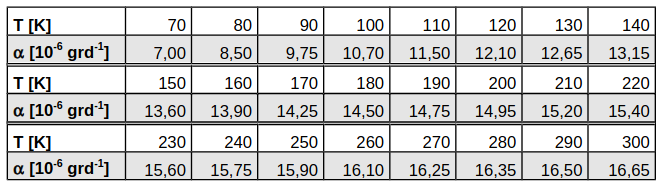
\includegraphics[width=\textwidth]{bilder/alpha.png}
   \caption{A table with the expansion coefficient dependent on the temperature.}
   \label{tab:alpha}
\end{figure}
